% Graphic for TeX using PGF
% Title: Z:\people\stephen\GlobalDocs\Projects\IPMAS\Architecture\Metric Taxonomy.dia
% Creator: Dia v0.97.2
% CreationDate: Thu Nov 01 16:39:04 2012
% For: stephen
% \usepackage{tikz}
% The following commands are not supported in PSTricks at present
% We define them conditionally, so when they are implemented,
% this pgf file will use them.
\ifx\du\undefined
  \newlength{\du}
\fi
\setlength{\du}{15\unitlength}
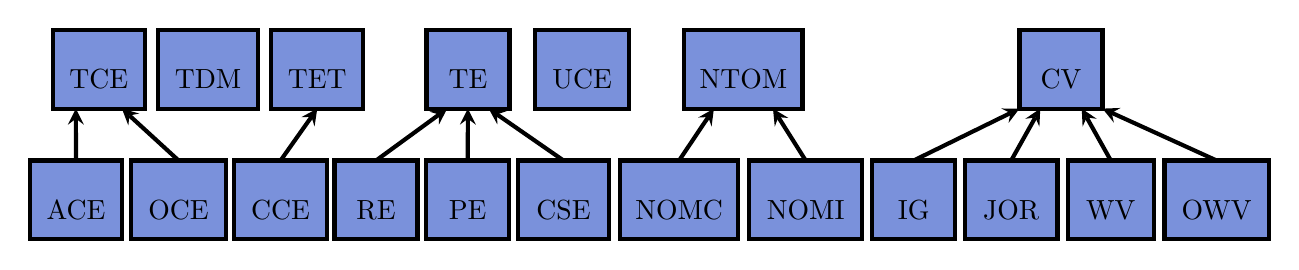
\begin{tikzpicture}
\pgftransformxscale{1.000000}
\pgftransformyscale{-1.000000}
\definecolor{dialinecolor}{rgb}{0.000000, 0.000000, 0.000000}
\pgfsetstrokecolor{dialinecolor}
\definecolor{dialinecolor}{rgb}{1.000000, 1.000000, 1.000000}
\pgfsetfillcolor{dialinecolor}
\definecolor{dialinecolor}{rgb}{0.478431, 0.568627, 0.858824}
\pgfsetfillcolor{dialinecolor}
\fill (1.257500\du,13.750000\du)--(1.257500\du,15.650000\du)--(3.487500\du,15.650000\du)--(3.487500\du,13.750000\du)--cycle;
\pgfsetlinewidth{0.100000\du}
\pgfsetdash{}{0pt}
\pgfsetdash{}{0pt}
\pgfsetmiterjoin
\definecolor{dialinecolor}{rgb}{0.000000, 0.000000, 0.000000}
\pgfsetstrokecolor{dialinecolor}
\draw (1.257500\du,13.750000\du)--(1.257500\du,15.650000\du)--(3.487500\du,15.650000\du)--(3.487500\du,13.750000\du)--cycle;
% setfont left to latex
\definecolor{dialinecolor}{rgb}{0.000000, 0.000000, 0.000000}
\pgfsetstrokecolor{dialinecolor}
\node at (2.372500\du,14.940000\du){ACE};
\definecolor{dialinecolor}{rgb}{0.478431, 0.568627, 0.858824}
\pgfsetfillcolor{dialinecolor}
\fill (3.694840\du,13.750000\du)--(3.694840\du,15.650000\du)--(5.992340\du,15.650000\du)--(5.992340\du,13.750000\du)--cycle;
\pgfsetlinewidth{0.100000\du}
\pgfsetdash{}{0pt}
\pgfsetdash{}{0pt}
\pgfsetmiterjoin
\definecolor{dialinecolor}{rgb}{0.000000, 0.000000, 0.000000}
\pgfsetstrokecolor{dialinecolor}
\draw (3.694840\du,13.750000\du)--(3.694840\du,15.650000\du)--(5.992340\du,15.650000\du)--(5.992340\du,13.750000\du)--cycle;
% setfont left to latex
\definecolor{dialinecolor}{rgb}{0.000000, 0.000000, 0.000000}
\pgfsetstrokecolor{dialinecolor}
\node at (4.843590\du,14.940000\du){OCE};
\definecolor{dialinecolor}{rgb}{0.478431, 0.568627, 0.858824}
\pgfsetfillcolor{dialinecolor}
\fill (1.812500\du,10.600000\du)--(1.812500\du,12.500000\du)--(4.032500\du,12.500000\du)--(4.032500\du,10.600000\du)--cycle;
\pgfsetlinewidth{0.100000\du}
\pgfsetdash{}{0pt}
\pgfsetdash{}{0pt}
\pgfsetmiterjoin
\definecolor{dialinecolor}{rgb}{0.000000, 0.000000, 0.000000}
\pgfsetstrokecolor{dialinecolor}
\draw (1.812500\du,10.600000\du)--(1.812500\du,12.500000\du)--(4.032500\du,12.500000\du)--(4.032500\du,10.600000\du)--cycle;
% setfont left to latex
\definecolor{dialinecolor}{rgb}{0.000000, 0.000000, 0.000000}
\pgfsetstrokecolor{dialinecolor}
\node at (2.922500\du,11.790000\du){TCE};
\definecolor{dialinecolor}{rgb}{0.478431, 0.568627, 0.858824}
\pgfsetfillcolor{dialinecolor}
\fill (4.352030\du,10.600000\du)--(4.352030\du,12.500000\du)--(6.754530\du,12.500000\du)--(6.754530\du,10.600000\du)--cycle;
\pgfsetlinewidth{0.100000\du}
\pgfsetdash{}{0pt}
\pgfsetdash{}{0pt}
\pgfsetmiterjoin
\definecolor{dialinecolor}{rgb}{0.000000, 0.000000, 0.000000}
\pgfsetstrokecolor{dialinecolor}
\draw (4.352030\du,10.600000\du)--(4.352030\du,12.500000\du)--(6.754530\du,12.500000\du)--(6.754530\du,10.600000\du)--cycle;
% setfont left to latex
\definecolor{dialinecolor}{rgb}{0.000000, 0.000000, 0.000000}
\pgfsetstrokecolor{dialinecolor}
\node at (5.553280\du,11.790000\du){TDM};
\definecolor{dialinecolor}{rgb}{0.478431, 0.568627, 0.858824}
\pgfsetfillcolor{dialinecolor}
\fill (7.074060\du,10.600000\du)--(7.074060\du,12.500000\du)--(9.294060\du,12.500000\du)--(9.294060\du,10.600000\du)--cycle;
\pgfsetlinewidth{0.100000\du}
\pgfsetdash{}{0pt}
\pgfsetdash{}{0pt}
\pgfsetmiterjoin
\definecolor{dialinecolor}{rgb}{0.000000, 0.000000, 0.000000}
\pgfsetstrokecolor{dialinecolor}
\draw (7.074060\du,10.600000\du)--(7.074060\du,12.500000\du)--(9.294060\du,12.500000\du)--(9.294060\du,10.600000\du)--cycle;
% setfont left to latex
\definecolor{dialinecolor}{rgb}{0.000000, 0.000000, 0.000000}
\pgfsetstrokecolor{dialinecolor}
\node at (8.184060\du,11.790000\du){TET};
\definecolor{dialinecolor}{rgb}{0.478431, 0.568627, 0.858824}
\pgfsetfillcolor{dialinecolor}
\fill (8.599690\du,13.750000\du)--(8.599690\du,15.650000\du)--(10.599690\du,15.650000\du)--(10.599690\du,13.750000\du)--cycle;
\pgfsetlinewidth{0.100000\du}
\pgfsetdash{}{0pt}
\pgfsetdash{}{0pt}
\pgfsetmiterjoin
\definecolor{dialinecolor}{rgb}{0.000000, 0.000000, 0.000000}
\pgfsetstrokecolor{dialinecolor}
\draw (8.599690\du,13.750000\du)--(8.599690\du,15.650000\du)--(10.599690\du,15.650000\du)--(10.599690\du,13.750000\du)--cycle;
% setfont left to latex
\definecolor{dialinecolor}{rgb}{0.000000, 0.000000, 0.000000}
\pgfsetstrokecolor{dialinecolor}
\node at (9.599690\du,14.940000\du){RE};
\definecolor{dialinecolor}{rgb}{0.478431, 0.568627, 0.858824}
\pgfsetfillcolor{dialinecolor}
\fill (10.807000\du,13.750000\du)--(10.807000\du,15.650000\du)--(12.807000\du,15.650000\du)--(12.807000\du,13.750000\du)--cycle;
\pgfsetlinewidth{0.100000\du}
\pgfsetdash{}{0pt}
\pgfsetdash{}{0pt}
\pgfsetmiterjoin
\definecolor{dialinecolor}{rgb}{0.000000, 0.000000, 0.000000}
\pgfsetstrokecolor{dialinecolor}
\draw (10.807000\du,13.750000\du)--(10.807000\du,15.650000\du)--(12.807000\du,15.650000\du)--(12.807000\du,13.750000\du)--cycle;
% setfont left to latex
\definecolor{dialinecolor}{rgb}{0.000000, 0.000000, 0.000000}
\pgfsetstrokecolor{dialinecolor}
\node at (11.807000\du,14.940000\du){PE};
\definecolor{dialinecolor}{rgb}{0.478431, 0.568627, 0.858824}
\pgfsetfillcolor{dialinecolor}
\fill (13.014400\du,13.750000\du)--(13.014400\du,15.650000\du)--(15.216900\du,15.650000\du)--(15.216900\du,13.750000\du)--cycle;
\pgfsetlinewidth{0.100000\du}
\pgfsetdash{}{0pt}
\pgfsetdash{}{0pt}
\pgfsetmiterjoin
\definecolor{dialinecolor}{rgb}{0.000000, 0.000000, 0.000000}
\pgfsetstrokecolor{dialinecolor}
\draw (13.014400\du,13.750000\du)--(13.014400\du,15.650000\du)--(15.216900\du,15.650000\du)--(15.216900\du,13.750000\du)--cycle;
% setfont left to latex
\definecolor{dialinecolor}{rgb}{0.000000, 0.000000, 0.000000}
\pgfsetstrokecolor{dialinecolor}
\node at (14.115650\du,14.940000\du){CSE};
\definecolor{dialinecolor}{rgb}{0.478431, 0.568627, 0.858824}
\pgfsetfillcolor{dialinecolor}
\fill (10.813600\du,10.600000\du)--(10.813600\du,12.500000\du)--(12.813600\du,12.500000\du)--(12.813600\du,10.600000\du)--cycle;
\pgfsetlinewidth{0.100000\du}
\pgfsetdash{}{0pt}
\pgfsetdash{}{0pt}
\pgfsetmiterjoin
\definecolor{dialinecolor}{rgb}{0.000000, 0.000000, 0.000000}
\pgfsetstrokecolor{dialinecolor}
\draw (10.813600\du,10.600000\du)--(10.813600\du,12.500000\du)--(12.813600\du,12.500000\du)--(12.813600\du,10.600000\du)--cycle;
% setfont left to latex
\definecolor{dialinecolor}{rgb}{0.000000, 0.000000, 0.000000}
\pgfsetstrokecolor{dialinecolor}
\node at (11.813600\du,11.790000\du){TE};
\definecolor{dialinecolor}{rgb}{0.478431, 0.568627, 0.858824}
\pgfsetfillcolor{dialinecolor}
\fill (13.433100\du,10.600000\du)--(13.433100\du,12.500000\du)--(15.698100\du,12.500000\du)--(15.698100\du,10.600000\du)--cycle;
\pgfsetlinewidth{0.100000\du}
\pgfsetdash{}{0pt}
\pgfsetdash{}{0pt}
\pgfsetmiterjoin
\definecolor{dialinecolor}{rgb}{0.000000, 0.000000, 0.000000}
\pgfsetstrokecolor{dialinecolor}
\draw (13.433100\du,10.600000\du)--(13.433100\du,12.500000\du)--(15.698100\du,12.500000\du)--(15.698100\du,10.600000\du)--cycle;
% setfont left to latex
\definecolor{dialinecolor}{rgb}{0.000000, 0.000000, 0.000000}
\pgfsetstrokecolor{dialinecolor}
\node at (14.565600\du,11.790000\du){UCE};
\pgfsetlinewidth{0.100000\du}
\pgfsetdash{}{0pt}
\pgfsetdash{}{0pt}
\pgfsetbuttcap
{
\definecolor{dialinecolor}{rgb}{0.000000, 0.000000, 0.000000}
\pgfsetfillcolor{dialinecolor}
% was here!!!
\pgfsetarrowsend{stealth}
\definecolor{dialinecolor}{rgb}{0.000000, 0.000000, 0.000000}
\pgfsetstrokecolor{dialinecolor}
\draw (2.372500\du,13.750000\du)--(2.367500\du,12.500000\du);
}
\pgfsetlinewidth{0.100000\du}
\pgfsetdash{}{0pt}
\pgfsetdash{}{0pt}
\pgfsetbuttcap
{
\definecolor{dialinecolor}{rgb}{0.000000, 0.000000, 0.000000}
\pgfsetfillcolor{dialinecolor}
% was here!!!
\pgfsetarrowsend{stealth}
\definecolor{dialinecolor}{rgb}{0.000000, 0.000000, 0.000000}
\pgfsetstrokecolor{dialinecolor}
\draw (4.843590\du,13.750000\du)--(3.477500\du,12.500000\du);
}
\pgfsetlinewidth{0.100000\du}
\pgfsetdash{}{0pt}
\pgfsetdash{}{0pt}
\pgfsetbuttcap
{
\definecolor{dialinecolor}{rgb}{0.000000, 0.000000, 0.000000}
\pgfsetfillcolor{dialinecolor}
% was here!!!
\pgfsetarrowsend{stealth}
\definecolor{dialinecolor}{rgb}{0.000000, 0.000000, 0.000000}
\pgfsetstrokecolor{dialinecolor}
\draw (9.599690\du,13.750000\du)--(11.313600\du,12.500000\du);
}
\pgfsetlinewidth{0.100000\du}
\pgfsetdash{}{0pt}
\pgfsetdash{}{0pt}
\pgfsetbuttcap
{
\definecolor{dialinecolor}{rgb}{0.000000, 0.000000, 0.000000}
\pgfsetfillcolor{dialinecolor}
% was here!!!
\pgfsetarrowsend{stealth}
\definecolor{dialinecolor}{rgb}{0.000000, 0.000000, 0.000000}
\pgfsetstrokecolor{dialinecolor}
\draw (11.807000\du,13.750000\du)--(11.813600\du,12.500000\du);
}
\pgfsetlinewidth{0.100000\du}
\pgfsetdash{}{0pt}
\pgfsetdash{}{0pt}
\pgfsetbuttcap
{
\definecolor{dialinecolor}{rgb}{0.000000, 0.000000, 0.000000}
\pgfsetfillcolor{dialinecolor}
% was here!!!
\pgfsetarrowsend{stealth}
\definecolor{dialinecolor}{rgb}{0.000000, 0.000000, 0.000000}
\pgfsetstrokecolor{dialinecolor}
\draw (14.115650\du,13.750000\du)--(12.313600\du,12.500000\du);
}
\definecolor{dialinecolor}{rgb}{0.478431, 0.568627, 0.858824}
\pgfsetfillcolor{dialinecolor}
\fill (6.185000\du,13.750000\du)--(6.185000\du,15.650000\du)--(8.415000\du,15.650000\du)--(8.415000\du,13.750000\du)--cycle;
\pgfsetlinewidth{0.100000\du}
\pgfsetdash{}{0pt}
\pgfsetdash{}{0pt}
\pgfsetmiterjoin
\definecolor{dialinecolor}{rgb}{0.000000, 0.000000, 0.000000}
\pgfsetstrokecolor{dialinecolor}
\draw (6.185000\du,13.750000\du)--(6.185000\du,15.650000\du)--(8.415000\du,15.650000\du)--(8.415000\du,13.750000\du)--cycle;
% setfont left to latex
\definecolor{dialinecolor}{rgb}{0.000000, 0.000000, 0.000000}
\pgfsetstrokecolor{dialinecolor}
\node at (7.300000\du,14.940000\du){CCE};
\pgfsetlinewidth{0.100000\du}
\pgfsetdash{}{0pt}
\pgfsetdash{}{0pt}
\pgfsetbuttcap
{
\definecolor{dialinecolor}{rgb}{0.000000, 0.000000, 0.000000}
\pgfsetfillcolor{dialinecolor}
% was here!!!
\pgfsetarrowsend{stealth}
\definecolor{dialinecolor}{rgb}{0.000000, 0.000000, 0.000000}
\pgfsetstrokecolor{dialinecolor}
\draw (7.300000\du,13.750000\du)--(8.184060\du,12.500000\du);
}
\definecolor{dialinecolor}{rgb}{0.478431, 0.568627, 0.858824}
\pgfsetfillcolor{dialinecolor}
\fill (15.471250\du,13.750000\du)--(15.471250\du,15.650000\du)--(18.328750\du,15.650000\du)--(18.328750\du,13.750000\du)--cycle;
\pgfsetlinewidth{0.100000\du}
\pgfsetdash{}{0pt}
\pgfsetdash{}{0pt}
\pgfsetmiterjoin
\definecolor{dialinecolor}{rgb}{0.000000, 0.000000, 0.000000}
\pgfsetstrokecolor{dialinecolor}
\draw (15.471250\du,13.750000\du)--(15.471250\du,15.650000\du)--(18.328750\du,15.650000\du)--(18.328750\du,13.750000\du)--cycle;
% setfont left to latex
\definecolor{dialinecolor}{rgb}{0.000000, 0.000000, 0.000000}
\pgfsetstrokecolor{dialinecolor}
\node at (16.900000\du,14.940000\du){NOMC};
\definecolor{dialinecolor}{rgb}{0.478431, 0.568627, 0.858824}
\pgfsetfillcolor{dialinecolor}
\fill (18.593750\du,13.750000\du)--(18.593750\du,15.650000\du)--(21.306250\du,15.650000\du)--(21.306250\du,13.750000\du)--cycle;
\pgfsetlinewidth{0.100000\du}
\pgfsetdash{}{0pt}
\pgfsetdash{}{0pt}
\pgfsetmiterjoin
\definecolor{dialinecolor}{rgb}{0.000000, 0.000000, 0.000000}
\pgfsetstrokecolor{dialinecolor}
\draw (18.593750\du,13.750000\du)--(18.593750\du,15.650000\du)--(21.306250\du,15.650000\du)--(21.306250\du,13.750000\du)--cycle;
% setfont left to latex
\definecolor{dialinecolor}{rgb}{0.000000, 0.000000, 0.000000}
\pgfsetstrokecolor{dialinecolor}
\node at (19.950000\du,14.940000\du){NOMI};
\definecolor{dialinecolor}{rgb}{0.478431, 0.568627, 0.858824}
\pgfsetfillcolor{dialinecolor}
\fill (17.026250\du,10.600000\du)--(17.026250\du,12.500000\du)--(19.873750\du,12.500000\du)--(19.873750\du,10.600000\du)--cycle;
\pgfsetlinewidth{0.100000\du}
\pgfsetdash{}{0pt}
\pgfsetdash{}{0pt}
\pgfsetmiterjoin
\definecolor{dialinecolor}{rgb}{0.000000, 0.000000, 0.000000}
\pgfsetstrokecolor{dialinecolor}
\draw (17.026250\du,10.600000\du)--(17.026250\du,12.500000\du)--(19.873750\du,12.500000\du)--(19.873750\du,10.600000\du)--cycle;
% setfont left to latex
\definecolor{dialinecolor}{rgb}{0.000000, 0.000000, 0.000000}
\pgfsetstrokecolor{dialinecolor}
\node at (18.450000\du,11.790000\du){NTOM};
\definecolor{dialinecolor}{rgb}{0.478431, 0.568627, 0.858824}
\pgfsetfillcolor{dialinecolor}
\fill (21.550000\du,13.750000\du)--(21.550000\du,15.650000\du)--(23.550000\du,15.650000\du)--(23.550000\du,13.750000\du)--cycle;
\pgfsetlinewidth{0.100000\du}
\pgfsetdash{}{0pt}
\pgfsetdash{}{0pt}
\pgfsetmiterjoin
\definecolor{dialinecolor}{rgb}{0.000000, 0.000000, 0.000000}
\pgfsetstrokecolor{dialinecolor}
\draw (21.550000\du,13.750000\du)--(21.550000\du,15.650000\du)--(23.550000\du,15.650000\du)--(23.550000\du,13.750000\du)--cycle;
% setfont left to latex
\definecolor{dialinecolor}{rgb}{0.000000, 0.000000, 0.000000}
\pgfsetstrokecolor{dialinecolor}
\node at (22.550000\du,14.940000\du){IG};
\definecolor{dialinecolor}{rgb}{0.478431, 0.568627, 0.858824}
\pgfsetfillcolor{dialinecolor}
\fill (23.783750\du,13.750000\du)--(23.783750\du,15.650000\du)--(26.016250\du,15.650000\du)--(26.016250\du,13.750000\du)--cycle;
\pgfsetlinewidth{0.100000\du}
\pgfsetdash{}{0pt}
\pgfsetdash{}{0pt}
\pgfsetmiterjoin
\definecolor{dialinecolor}{rgb}{0.000000, 0.000000, 0.000000}
\pgfsetstrokecolor{dialinecolor}
\draw (23.783750\du,13.750000\du)--(23.783750\du,15.650000\du)--(26.016250\du,15.650000\du)--(26.016250\du,13.750000\du)--cycle;
% setfont left to latex
\definecolor{dialinecolor}{rgb}{0.000000, 0.000000, 0.000000}
\pgfsetstrokecolor{dialinecolor}
\node at (24.900000\du,14.940000\du){JOR};
\definecolor{dialinecolor}{rgb}{0.478431, 0.568627, 0.858824}
\pgfsetfillcolor{dialinecolor}
\fill (26.268750\du,13.750000\du)--(26.268750\du,15.650000\du)--(28.331250\du,15.650000\du)--(28.331250\du,13.750000\du)--cycle;
\pgfsetlinewidth{0.100000\du}
\pgfsetdash{}{0pt}
\pgfsetdash{}{0pt}
\pgfsetmiterjoin
\definecolor{dialinecolor}{rgb}{0.000000, 0.000000, 0.000000}
\pgfsetstrokecolor{dialinecolor}
\draw (26.268750\du,13.750000\du)--(26.268750\du,15.650000\du)--(28.331250\du,15.650000\du)--(28.331250\du,13.750000\du)--cycle;
% setfont left to latex
\definecolor{dialinecolor}{rgb}{0.000000, 0.000000, 0.000000}
\pgfsetstrokecolor{dialinecolor}
\node at (27.300000\du,14.940000\du){WV};
\definecolor{dialinecolor}{rgb}{0.478431, 0.568627, 0.858824}
\pgfsetfillcolor{dialinecolor}
\fill (28.593750\du,13.750000\du)--(28.593750\du,15.650000\du)--(31.106250\du,15.650000\du)--(31.106250\du,13.750000\du)--cycle;
\pgfsetlinewidth{0.100000\du}
\pgfsetdash{}{0pt}
\pgfsetdash{}{0pt}
\pgfsetmiterjoin
\definecolor{dialinecolor}{rgb}{0.000000, 0.000000, 0.000000}
\pgfsetstrokecolor{dialinecolor}
\draw (28.593750\du,13.750000\du)--(28.593750\du,15.650000\du)--(31.106250\du,15.650000\du)--(31.106250\du,13.750000\du)--cycle;
% setfont left to latex
\definecolor{dialinecolor}{rgb}{0.000000, 0.000000, 0.000000}
\pgfsetstrokecolor{dialinecolor}
\node at (29.850000\du,14.940000\du){OWV};
\definecolor{dialinecolor}{rgb}{0.478431, 0.568627, 0.858824}
\pgfsetfillcolor{dialinecolor}
\fill (25.100000\du,10.600000\du)--(25.100000\du,12.500000\du)--(27.100000\du,12.500000\du)--(27.100000\du,10.600000\du)--cycle;
\pgfsetlinewidth{0.100000\du}
\pgfsetdash{}{0pt}
\pgfsetdash{}{0pt}
\pgfsetmiterjoin
\definecolor{dialinecolor}{rgb}{0.000000, 0.000000, 0.000000}
\pgfsetstrokecolor{dialinecolor}
\draw (25.100000\du,10.600000\du)--(25.100000\du,12.500000\du)--(27.100000\du,12.500000\du)--(27.100000\du,10.600000\du)--cycle;
% setfont left to latex
\definecolor{dialinecolor}{rgb}{0.000000, 0.000000, 0.000000}
\pgfsetstrokecolor{dialinecolor}
\node at (26.100000\du,11.790000\du){CV};
\pgfsetlinewidth{0.100000\du}
\pgfsetdash{}{0pt}
\pgfsetdash{}{0pt}
\pgfsetbuttcap
{
\definecolor{dialinecolor}{rgb}{0.000000, 0.000000, 0.000000}
\pgfsetfillcolor{dialinecolor}
% was here!!!
\pgfsetarrowsend{stealth}
\definecolor{dialinecolor}{rgb}{0.000000, 0.000000, 0.000000}
\pgfsetstrokecolor{dialinecolor}
\draw (16.900000\du,13.750000\du)--(17.738125\du,12.500000\du);
}
\pgfsetlinewidth{0.100000\du}
\pgfsetdash{}{0pt}
\pgfsetdash{}{0pt}
\pgfsetbuttcap
{
\definecolor{dialinecolor}{rgb}{0.000000, 0.000000, 0.000000}
\pgfsetfillcolor{dialinecolor}
% was here!!!
\pgfsetarrowsend{stealth}
\definecolor{dialinecolor}{rgb}{0.000000, 0.000000, 0.000000}
\pgfsetstrokecolor{dialinecolor}
\draw (19.950000\du,13.750000\du)--(19.161875\du,12.500000\du);
}
\pgfsetlinewidth{0.100000\du}
\pgfsetdash{}{0pt}
\pgfsetdash{}{0pt}
\pgfsetbuttcap
{
\definecolor{dialinecolor}{rgb}{0.000000, 0.000000, 0.000000}
\pgfsetfillcolor{dialinecolor}
% was here!!!
\pgfsetarrowsend{stealth}
\definecolor{dialinecolor}{rgb}{0.000000, 0.000000, 0.000000}
\pgfsetstrokecolor{dialinecolor}
\draw (22.550000\du,13.750000\du)--(25.100000\du,12.500000\du);
}
\pgfsetlinewidth{0.100000\du}
\pgfsetdash{}{0pt}
\pgfsetdash{}{0pt}
\pgfsetbuttcap
{
\definecolor{dialinecolor}{rgb}{0.000000, 0.000000, 0.000000}
\pgfsetfillcolor{dialinecolor}
% was here!!!
\pgfsetarrowsend{stealth}
\definecolor{dialinecolor}{rgb}{0.000000, 0.000000, 0.000000}
\pgfsetstrokecolor{dialinecolor}
\draw (24.900000\du,13.750000\du)--(25.600000\du,12.500000\du);
}
\pgfsetlinewidth{0.100000\du}
\pgfsetdash{}{0pt}
\pgfsetdash{}{0pt}
\pgfsetbuttcap
{
\definecolor{dialinecolor}{rgb}{0.000000, 0.000000, 0.000000}
\pgfsetfillcolor{dialinecolor}
% was here!!!
\pgfsetarrowsend{stealth}
\definecolor{dialinecolor}{rgb}{0.000000, 0.000000, 0.000000}
\pgfsetstrokecolor{dialinecolor}
\draw (27.300000\du,13.750000\du)--(26.600000\du,12.500000\du);
}
\pgfsetlinewidth{0.100000\du}
\pgfsetdash{}{0pt}
\pgfsetdash{}{0pt}
\pgfsetbuttcap
{
\definecolor{dialinecolor}{rgb}{0.000000, 0.000000, 0.000000}
\pgfsetfillcolor{dialinecolor}
% was here!!!
\pgfsetarrowsend{stealth}
\definecolor{dialinecolor}{rgb}{0.000000, 0.000000, 0.000000}
\pgfsetstrokecolor{dialinecolor}
\draw (29.850000\du,13.750000\du)--(27.100000\du,12.500000\du);
}
\end{tikzpicture}
